\documentclass[11pt]{article}
\usepackage{geometry,marginnote} % Pour passer au format A4
\geometry{hmargin=1cm, vmargin=1cm} % 

% Page et encodage
\usepackage[T1]{fontenc} % Use 8-bit encoding that has 256 glyphs
\usepackage[english,french]{babel} % Français et anglais
\usepackage[utf8]{inputenc} 

\usepackage{lmodern,numprint}
\setlength\parindent{0pt}

% Graphiques
\usepackage{graphicx,float,grffile,units}
\usepackage{tikz,pst-eucl,pst-plot,pstricks,pst-node,pstricks-add,pst-fun,pgfplots} 

% Maths et divers
\usepackage{amsmath,amsfonts,amssymb,amsthm,verbatim}
\usepackage{multicol,enumitem,url,eurosym,gensymb,tabularx}

\DeclareUnicodeCharacter{20AC}{\euro}



% Sections
\usepackage{sectsty} % Allows customizing section commands
\allsectionsfont{\centering \normalfont\scshape}

% Tête et pied de page
\usepackage{fancyhdr} \pagestyle{fancyplain} \fancyhead{} \fancyfoot{}

\renewcommand{\headrulewidth}{0pt} % Remove header underlines
\renewcommand{\footrulewidth}{0pt} % Remove footer underlines

\newcommand{\horrule}[1]{\rule{\linewidth}{#1}} % Create horizontal rule command with 1 argument of height

\newcommand{\Pointilles}[1][3]{%
  \multido{}{#1}{\makebox[\linewidth]{\dotfill}\\[\parskip]
}}

\newtheorem{Definition}{Définition}

\usepackage{siunitx}
\sisetup{
    detect-all,
    output-decimal-marker={,},
    group-minimum-digits = 3,
    group-separator={~},
    number-unit-separator={~},
    inter-unit-product={~}
}

\setlength{\columnseprule}{1pt}

\begin{document}

\textbf{Nom, Prénom :} \hspace{8cm} \textbf{Classe :} \hspace{3cm} \textbf{Date :}\\

\vspace{-0.5cm} \begin{center}
  \textit{La valeur morale ne peut pas être remplacée par la valeur intelligence et j'ajouterai : Dieu merci !}  - \textbf{Albert Einstein}
\end{center}

\begin{multicols}{2}

\textbf{Pb1 - Bateau}

\begin{figure}[H]
  \centering
  \includegraphics[width=0.6\linewidth]{4x10-trigonometrie/pb1.pdf}
\end{figure}

\begin{enumerate}
  \item Entre la tour et le phare, le bateau avance à la vitesse de $6m/s$ pendant 2min. \\
  Quelle est la distance ?
  \item Pour être en sécurité, le bateau doit être à une distance plus grande que $350m$ de la côté. \\
  Le bateau est-il en sécurité ?
\end{enumerate} \columnbreak

\Pointilles[17]

\end{multicols}

\textbf{Pb2 - Terre}

\begin{multicols}{2}

  \begin{figure}[H]
    \centering
    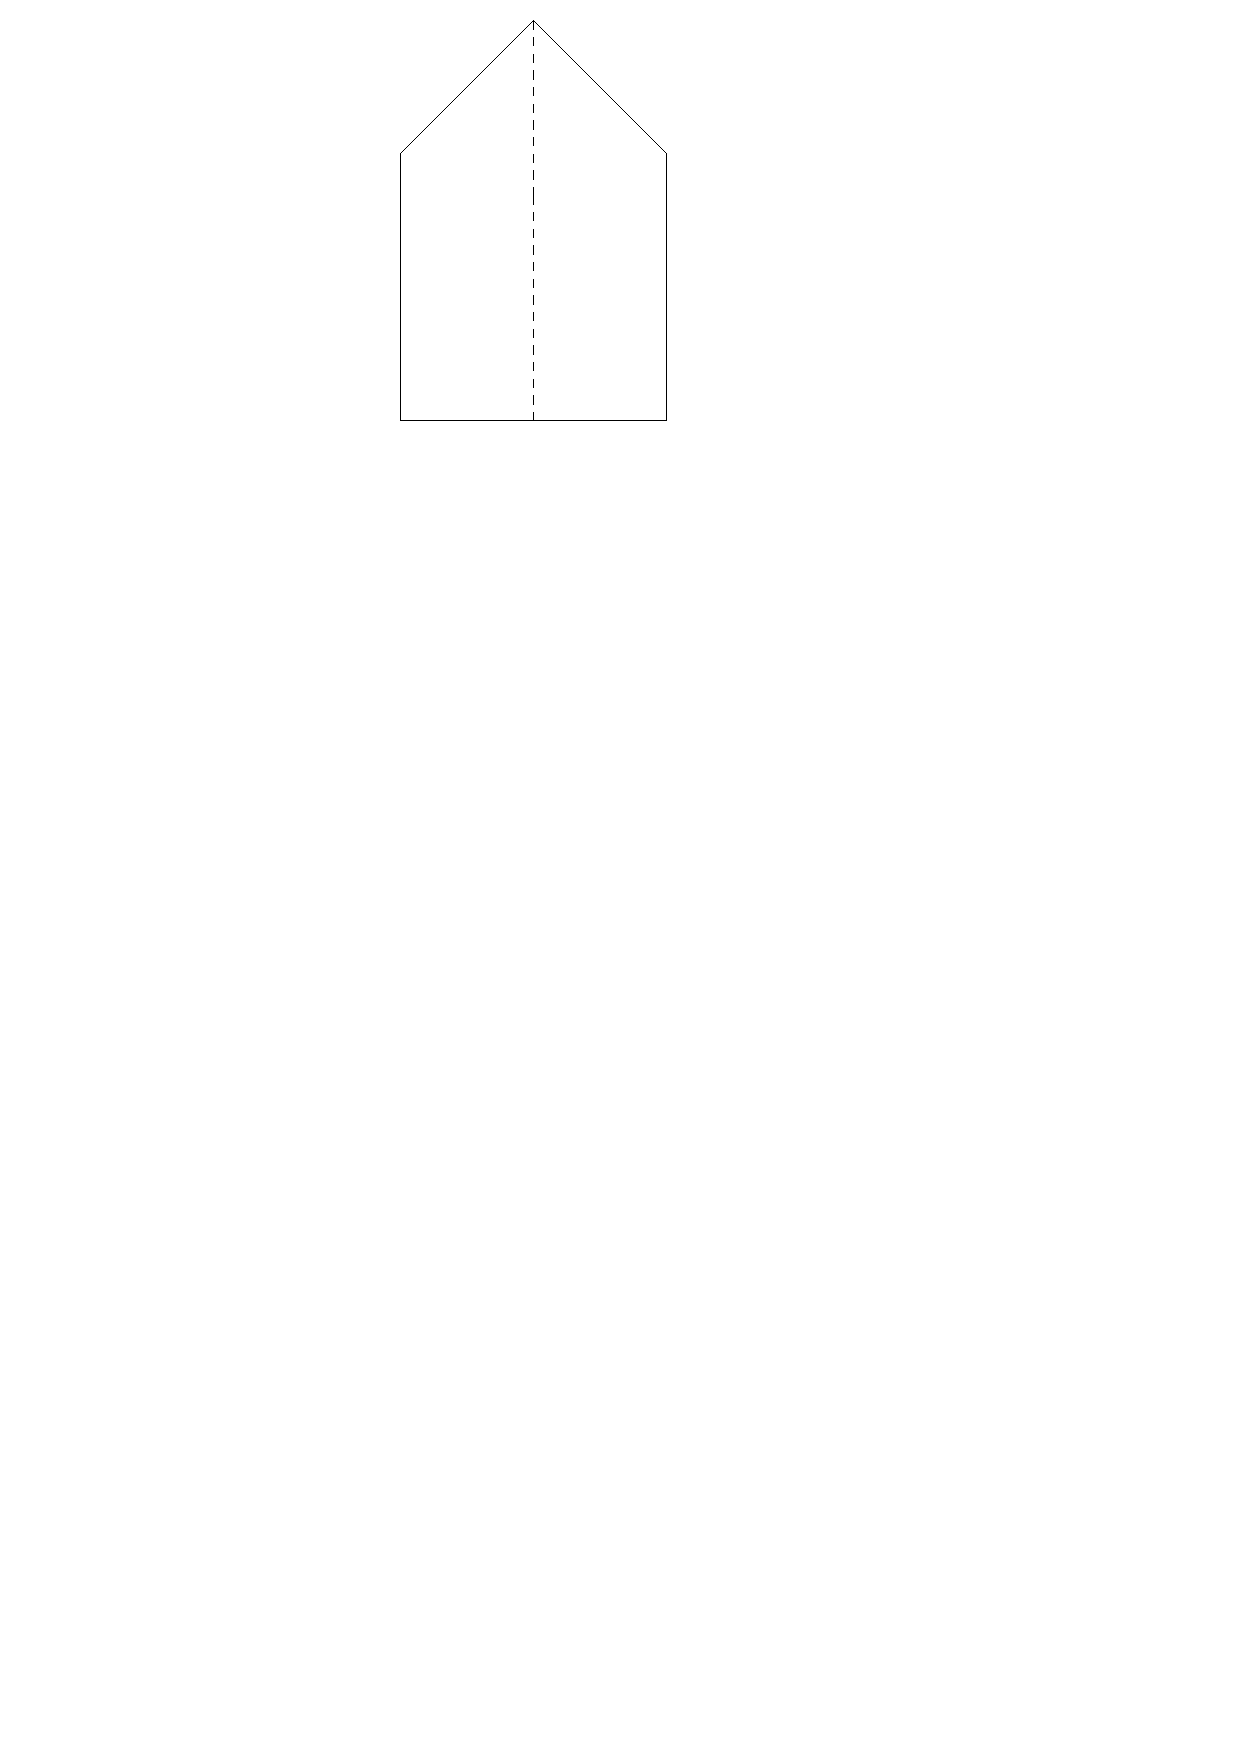
\includegraphics[width=0.6\linewidth]{4x10-trigonometrie/pb2.pdf}
  \end{figure}
  
  Le Rayon de la Terre est $6 371 km$. 
  \begin{enumerate}
    \item Calculer la distance AF.
    \item Calculer le périmètre du \textit{parallèle} passant par F.
    \item La terre fait un tour sur elle-même en 24h. \\
    Calculer la vitesse à lequel tourne le point F en une journée.
  \end{enumerate} \columnbreak

  \Pointilles[18]

\end{multicols}

\Pointilles[8]


\end{document}
